\documentclass{article}
\usepackage[margin=1in]{geometry}
\usepackage{amsmath}
\usepackage{amsfonts}
\usepackage{graphicx}
\usepackage{xcolor}
\usepackage{ulem}
\input{sym}


\title{ECE 498/598 Midterm 2 2023}
\date{Nov 8th, 2023}
\author{Instructor: Vikas Dhiman}

\newtheorem{prob}{Problem}
\newif\ifsol
\solfalse

\begin{document}
\maketitle
%$ \hat{\mathbf{w}} = \hat{\mathbf{k}} \times \frac{\mathbf{v}}{\|\mathbf{v}\|} $
%$ \|\hat{\mathbf{w}}\| = \|\hat{\mathbf{k}}\| \|\frac{\mathbf{v}}{\|\mathbf{v}\|}\| \sin(\phi) $. 

\begin{tabular}{p{0.5\linewidth}p{0.5\linewidth}}
  (1) Student name:& Student email: \\
\end{tabular}

\subsubsection*{About the exam}
\begin{enumerate}
  \item There are total 4 problems. You must attempt all 4.
  \item Maximum marks: 50.
  \item Maximum time allotted:  50 min
  \item Calculators are allowed.
  \item One US Letter size or A4 size cheat sheet (both-sides) is allowed.
\end{enumerate}

\begin{prob}
  Find the 4x4 transformation matrix $^1T_0$ that transforms coordinates from coordinate frame 1 to coordinate frame 0 (5 marks).\\
  \includegraphics[width=0.7\linewidth,trim=0 0 0 1in,clip]{./media/transformations.png}
\end{prob}
\newpage
.
\newpage

\begin{prob}
  Consider a coordinate system OUVW whose ordered set of basis vectors given by
  $\bfu = [3/7, 2/7, 6/7]^\top$, $\bfv = [2/7, 6/7, 3/7]^\top$ and $\bfw = [4,
  5, 6]^\top$.
  Another coordinate system OXYZ whose order set of basis vectors is, $\bfx =
  [2/7, 6/7, -3/7]^\top$, $\bfy = [-6/7, 3/7, 2/7]^\top$ and $\bfz = [3/7, 2/7, 6/7]^\top$.
  Find the rotation matrix $^{ouvw}R_{oxyz}$ that converts coordinates from frame OXYZ to frame OUVW. (10 marks)
\end{prob}
\newpage

\begin{prob}
  (Rodrigues formula) In the figure below, we are rotating point $\bfv$ around
  axis unit-vector $\hat{\bfk}$ by an angle $\theta$. A unit vector $\hat{\bfw}$ is
  perpendicular to the both $\bfv$ and $\hat{\bfk}$. Another vector $\bfv_{\perp}$ is the projection of $\bfv$ onto a plane that is perpendicular to $\hat{\bfk}$. Note that $\bfv_{\perp}$ is perpendicular to both $\hat{\bfw}$ and $\hat{\bfk}$. First, (a) write the
  unit-vector $\hat{\bfw}$ in terms of $\bfv$ and $\hat{\bfk}$.
  (b) Then write the vector (including the correct magnitude) $\bfv_\perp$ in terms of $\bfv$ and $\hat{\bfk}$.
  (c) A vector $\bfv_{\perp,\text{rot}}$ is obtained by rotating $\bfv_\perp$ by an angle $\theta$. Write the vector $\bfv_{\perp,\text{rot}}$ in terms of $\bfv_{\perp}$, $\hat{\bfw}$ and $\theta$. 
  (15 marks)\\
  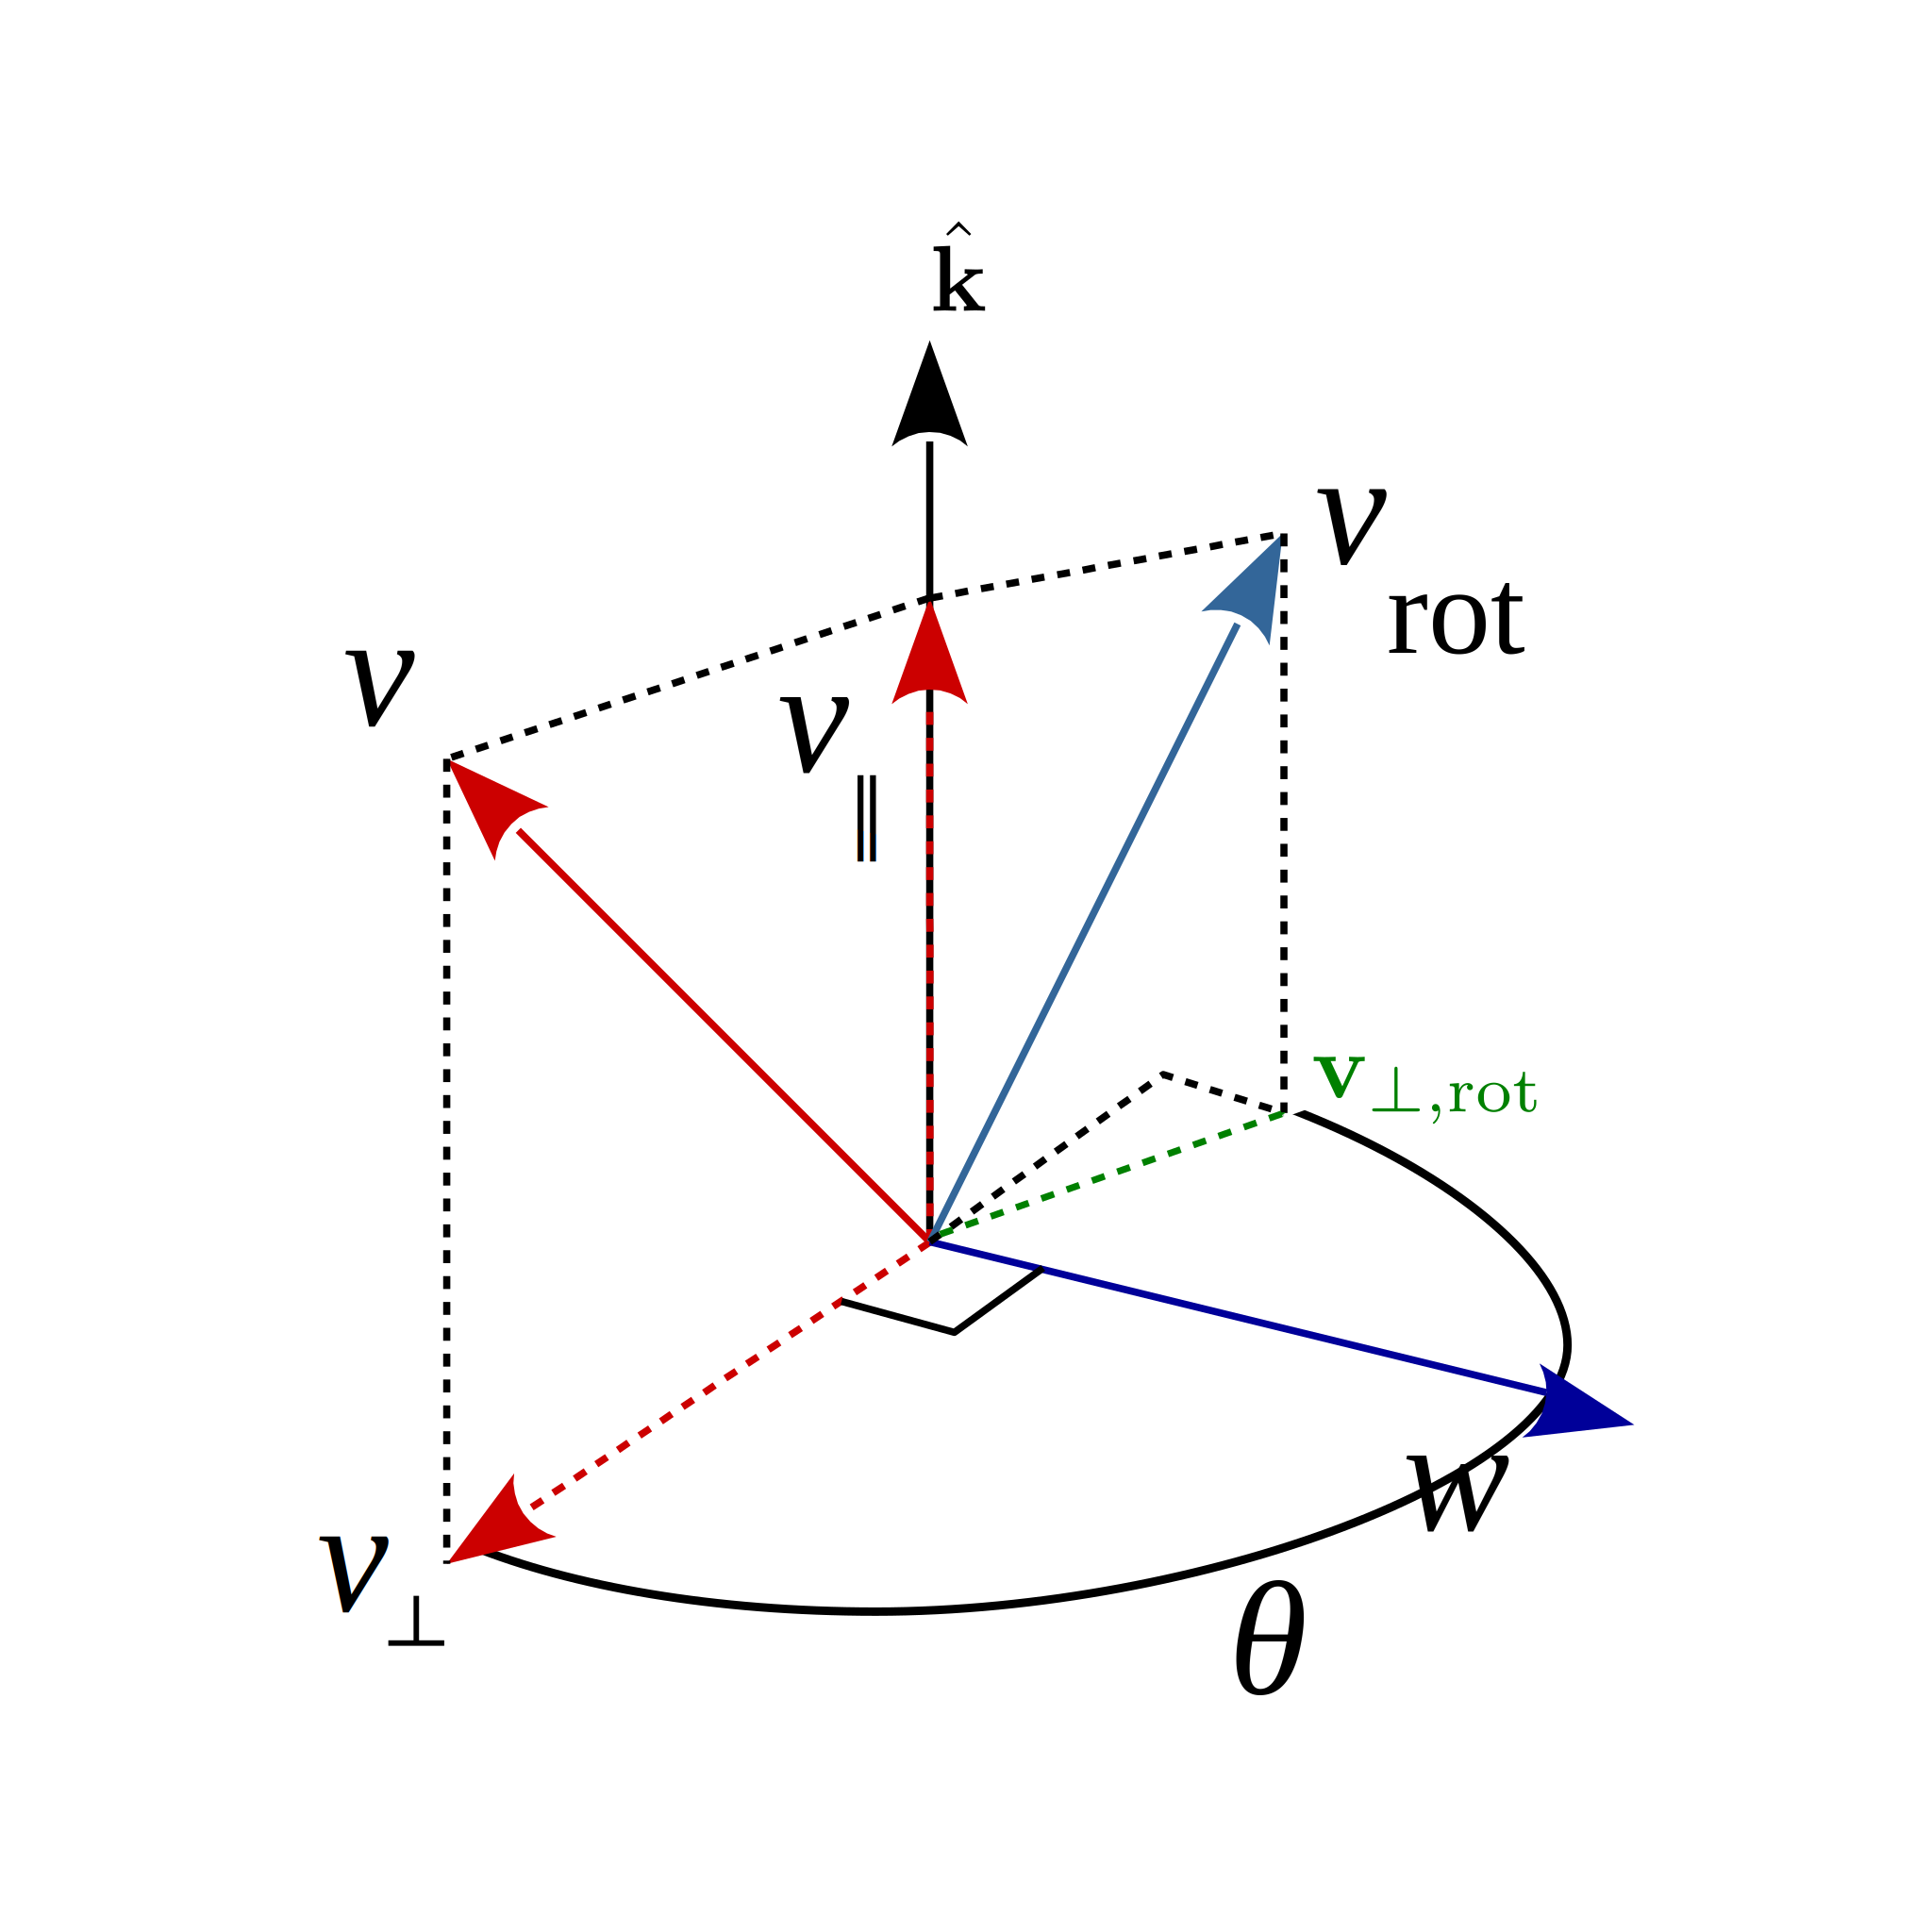
\includegraphics[width=0.5\linewidth]{media/Rodrigues-formula.pdf}
\end{prob}

\newpage

\begin{prob}
  The Euler angles of rotation YZX are given as $\theta$, $\phi$ and $\psi$.
  Derive the rotation matrix corresponding to the Euler angle representation $R = R_x(\psi) R_z(\phi) R_y(\theta)$. Also derive an expression to convert the rotation matrix back to Euler angles. (20 marks).
\end{prob}

\newpage

\end{document}
